There are 20 different amino acids to act as building blocks for proteins (Fig. \ref{fig:amino_acids}).
This alphabet displays diverse structural and chemical properties, 
giving proteins the ability to assume many functional roles.
Each amino acid consist of a central $\alpha$-carbon,
which is linked to four different groups:
an amino group,
a carboxylic acid group,
a hydrogen atom,
and one of the 20 possible sidechains.
A wide range of functional groups can be displayed on the sidechain,
including alcohols,
a thiol,
a thioether,
carboxylic acids,
and various basic groups.
Because these 20 unique amino acids,
each with their own physico-chemical properties,
can be ordered in numerous ways in a protein sequence, 
there is broad spectrum of protein functionality
(\cite{berg2015}).

~\begin{figure}[h!]
	~\begin{subfigure}[b]{0.70\linewidth}
		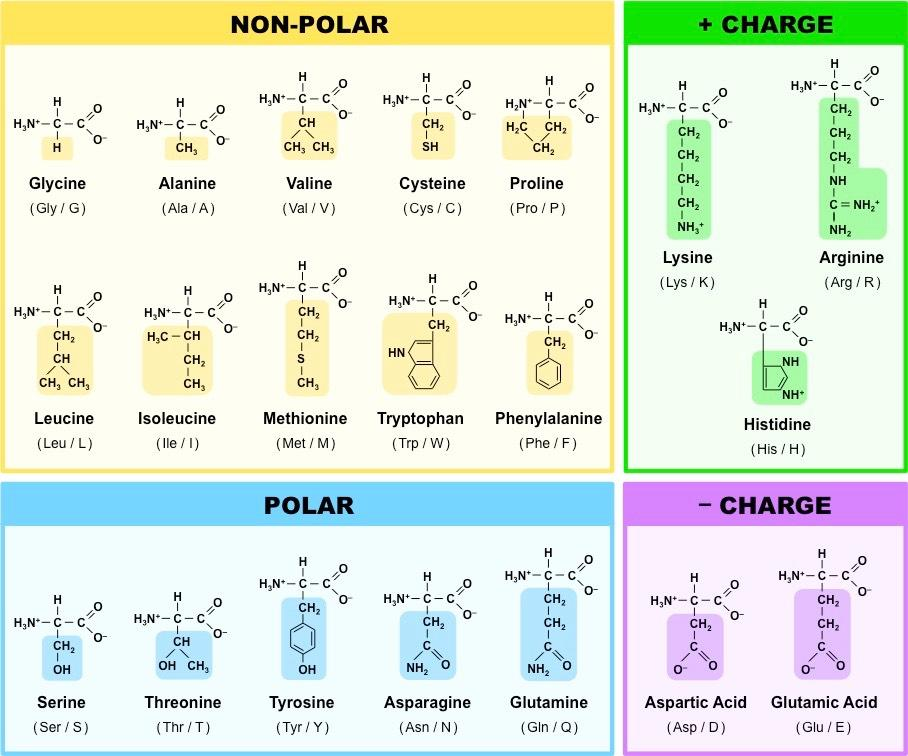
\includegraphics[width=\linewidth]{./literature_review/proteins/amino_acids/img/classification.jpg}
		\caption{\textbf{Classification}}
	~\end{subfigure}
	~\begin{subfigure}[b]{0.25\linewidth}
		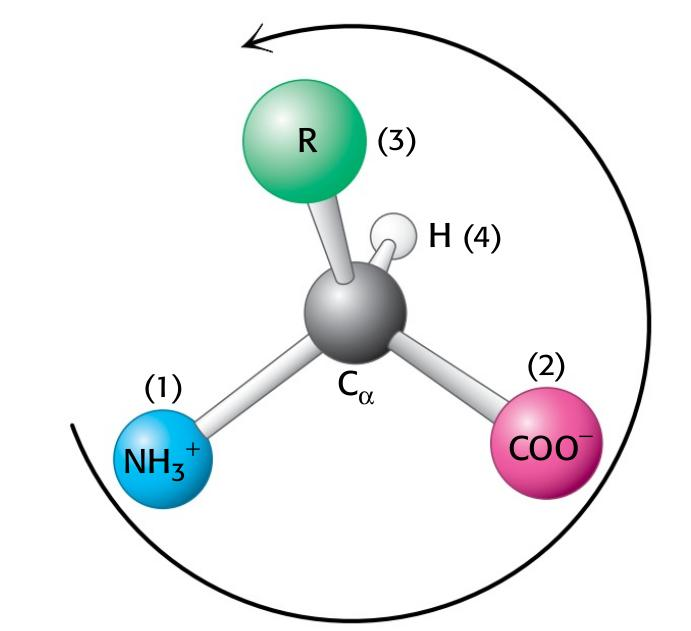
\includegraphics[width=\linewidth]{./literature_review/proteins/amino_acids/img/structure.jpg}
		\caption{\textbf{Structure}}
	~\end{subfigure}
	\caption{
		\textbf{Amino acids. a.}
	Amino acid classification by general chemical properties. 
	Each amino acid is depicted with its chemical structure, name, three-letter and one-letter code. 
	The sidechains are highlighted by a coloured frame 
	(from ib.bioninja.com.au).
		\textbf{b.}
	The general structure of an amino acid. 
	A central alpha-carbon is connected to 
	an amino group (blue),
	a carboxylic acid group (pink),
	an hydrogen atom (white),
	and a one of the 20 sidechains (green).
	(from \cite{berg2015}).
	}
	\label{fig:amino_acids}
~\end{figure}
